
\chapter{The HPS Apparatus}

%The HPS experiment engineering run was conducted in the Spring of 2015 at the
%Thomas Jefferson National Accelerator Facility (JLab) in Newport News, VA.  The
%HPS detector was installed within the Hall B alcove upstream of the Continuous 
%Electron Beam Accelerator Facility (CEBAF) Large Acceptance Spectrometer for 12
%GeV (CLAS12) detector.  HPS utilized CEBAF's high luminosity electron beam,
%operating at an energy of 1.056 GeV and current of 50 nA, incident on a thin
%(~0.125\% $X_{0}$) tungsten target to search for an $A'$ with a mass in the 
%range of 20 - 100 MeV.  

At the energies at which the HPS experiment is operating, the 
electroproduced $A'$ will carry most of the incident beam energy. Consequently,
the $A'$ decay products will be highly boosted, necessitating a detector with very
forward acceptance that can be placed in close proximity to the target.
Maximizing the acceptance requires placing the detector close to the beam plane,
encroaching on a ``dead zone'' which is occupied by an intense flux of multiple
Coulomb scattered beam particles along with radiative secondaries originating
from the target.  In order to avoid additional background from from beam gas
interactions, the detector needs to operate in vacuum. Finally, minimizing the
material budget of the active area of the detector is essential to reducing the
multiple scattering that dominates both the mass and vertex resolutions that
determine the experimental sensitivity.

These design principles led to the conception of the HPS detector.  
Specifically, HPS utilizes a compact, large acceptance forward spectrometer 
consisting of a silicon microstrip tracker (SVT) along with a lead tungstate
electromagnetic calorimeter (Ecal).  The SVT is installed inside of a vacuum
chamber and inside of an analyzing magnet immediately downstream of a thin
($0.125\%X_{0}$) tungsten target.
The Ecal is placed downstream of the tracker and provides the primary 
trigger for the experiment and is also used for electron identification. Together, 
both subsystems provide the complete kinematic information required to 
reconstruct heavy photons.

The HPS detector was installed and comissioned within the Hall B alcove at the
Thomas Jefferson National Accelerator Facility (JLab) in Newport News, VA early
in the Spring of 2015. Shortly after, an engineering run took place utilizing
the Continuous Electron Beam Accelerator Facility (CEBAF) operating at an 
energy 1.056 GeV and current of 50 nA.

The chapter that follows will detail various elements of the experiment.
It will begin with a discussion of CEBAF and continue with descriptions
of several beamline elements, SVT, Ecal and data aquisition system (DAQ).

\section{CEBAF}

CEBAF's ability to provide a nearly continuous, clean and intense electron
beam makes it ideal to search for heavy photons with weak couplings. Recently,
CEBAF underwent an upgrade that increased its maximum operating energy to 12
GeV and introduced a new experimental hall, Hall D, that will house the
GlueX detector \cite{Dudek:2012vr}.  The upgraded facility is now capable of 
delivering 11 GeV electron beams to the three existing experimental halls
(Hall A, B, C) and can use the 12 GeV electron beam to generate and deliver a 9
GeV photon beam to Hall D. 

As shown on Figure \ref{fig:cebaf}, achieving 12 GeV operation, required several
improvements to the accelerator \cite{Burkert:2012rh}. Central to the upgrade 
was the addition of 5 
cryomodules to each of the linacs.  Coupled with upgrades to the accelerator
magnets and power supplies, the additional cryomodules allowed each linac to
accelerate electrons at a rate of 2.2 GeV per pass up to a maximum of 5 passes.
\begin{figure}[h]
    \centering
    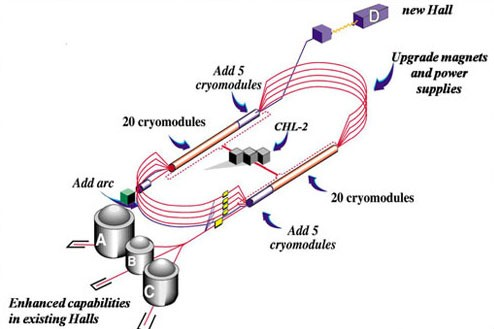
\includegraphics[width=0.9\textwidth]{images/cebaf.jpg}
    \caption{A diagram of the Thomas Jefferson National Accelerator Facility
             Continuous Electron Beam Accelerator Facility showing the 
             components that were upgraded as part of the 12 GeV Upgrade 
             program.}
    \label{fig:cebaf}
\end{figure}
Enabling four hall operation also required the addition of a new 750 MHz RF 
separator, a new laser to the electron source and a 10th arc which provides
the additional pass of acceleration that allows 
delivery of the maximum beam energy to Hall D.


\subsection{Electron Production and Injection}

%
%  Note: I need to make sure that this is still correct in the 12 GeV era.
%
The electrons injected into the accelerator were produced by photoemission from
a strained GaAs superlattice photocathode \cite{Maruyama:2004hx}.  Each of the 
four experimental halls has a dedicated gain-switched fiber coupled laser of
wavelength 1560 nm.  The lasers are frequency doubled in order to produce light
of wavelength of 780 nm, matching the band gap of the superlattice cathode. The
lasers are phased shifted and are each pulsed for $\approx$ 40 ps at the 
frequency of 499 MHz.  Since the operational frequency of the accelerator 
cryomodules is 1497 MHz, four hall operation requires subharmonics of 499 MHz to
be chosen.  This is achieved by ``cutting away'' pulses using an optical 
modulator \cite{Kazimi:2013yua}.


The photoemission electrons are released into an extremely high vacuum
environment at a pressure of $10^{-11}$ to $10^{-12}$ Torr.  The free electrons
are then delivered into the injector by a 100 keV electron gun.  The injector
itself then accelerates the electron bunches to an energy of 50 MeV 
%by 2 1/4 cryomodules 
before being delivered into the accelerator.

\subsection{Electron Acceleration}

The CEBAF accelerator is composed of two linacs arranged in a racetrack
configuration as shown on Fig \ref{fig:cebaf}. Each of the linacs consist
of 25 cryomodules, 5 of which were added as part of the upgrade.  The original
(new) cryomodules consist of 8 5-cell (7-cell) superconducting radio frequency
(RF) cavities made of ultra-pure Niobium (see Figure \ref{fig:cebaf_cavity}).  
The original cryomodules
\begin{figure}[h]
    \centering
    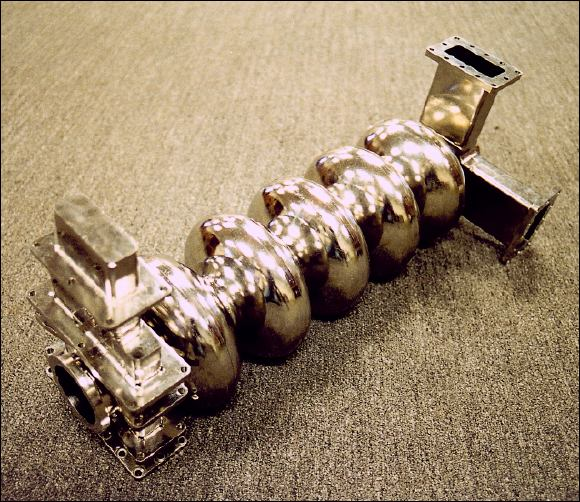
\includegraphics[width=0.7\textwidth]{images/cebaf_cavity.jpg}
    \caption{A 5-cell ultra-pure Niobium superconducting radio frequency cavity
             used to accelerate electrons at CEBAF.}
    \label{fig:cebaf_cavity}
\end{figure}
are capable of accelerating an electron upwards of 25 MeV while the newly installed
cryomodules can achieve an acceleration of 100 MeV.  This leads to an acceleration
of 1.1 GeV per linac and 2.2 GeV per pass. The 
number of passes depends on the energy requirements of the experiment taking place.
However, for electrons delivered to Halls A, B and C, the maximum amount of passes
is 5 while for Hall D, it's 5.5.

Electron bunches circulating the accelerator can be delivered to a Halls A, B
and C by an RF separator operating at a frequency of 499 MHz.  Delivery to Hall
D uses an RF separator of 750 MHz.

\subsection{Single Pass Operation For HPS}

During the Spring of 2015, HPS was prepared to run at a beam energy of 2.2 GeV,
in conjuction with the commissioning of the 750 MHz RF separator.
Unfortunately, an incident occured which resulted in the loss of the new CHL
required to operate the accelerator as a 12 GeV machine.
The loss caused the accelerator to 
fallback to 6 GeV operation using a single CHL.  As a result, HPS was given
the unique opportunity to run with a beam energy of 1.056 GeV allowing the
experiment to have sensitivity to the g-2 favored region of the mass-coupling
phase space.  

\section{Beamline}

\subsection{Layout}

The HPS experiment utilizes a three-magnet chicane system as shown on Figure 
\ref{fig:beamline}. The first and last dipoles of the chicane,  are used to bend
the beam into the HPS apparatus while the second dipole, the Hall B pair 
spectrometer, serves as the analyzing magnet of the experiment.  

\begin{sidewaysfigure}
    \centering
    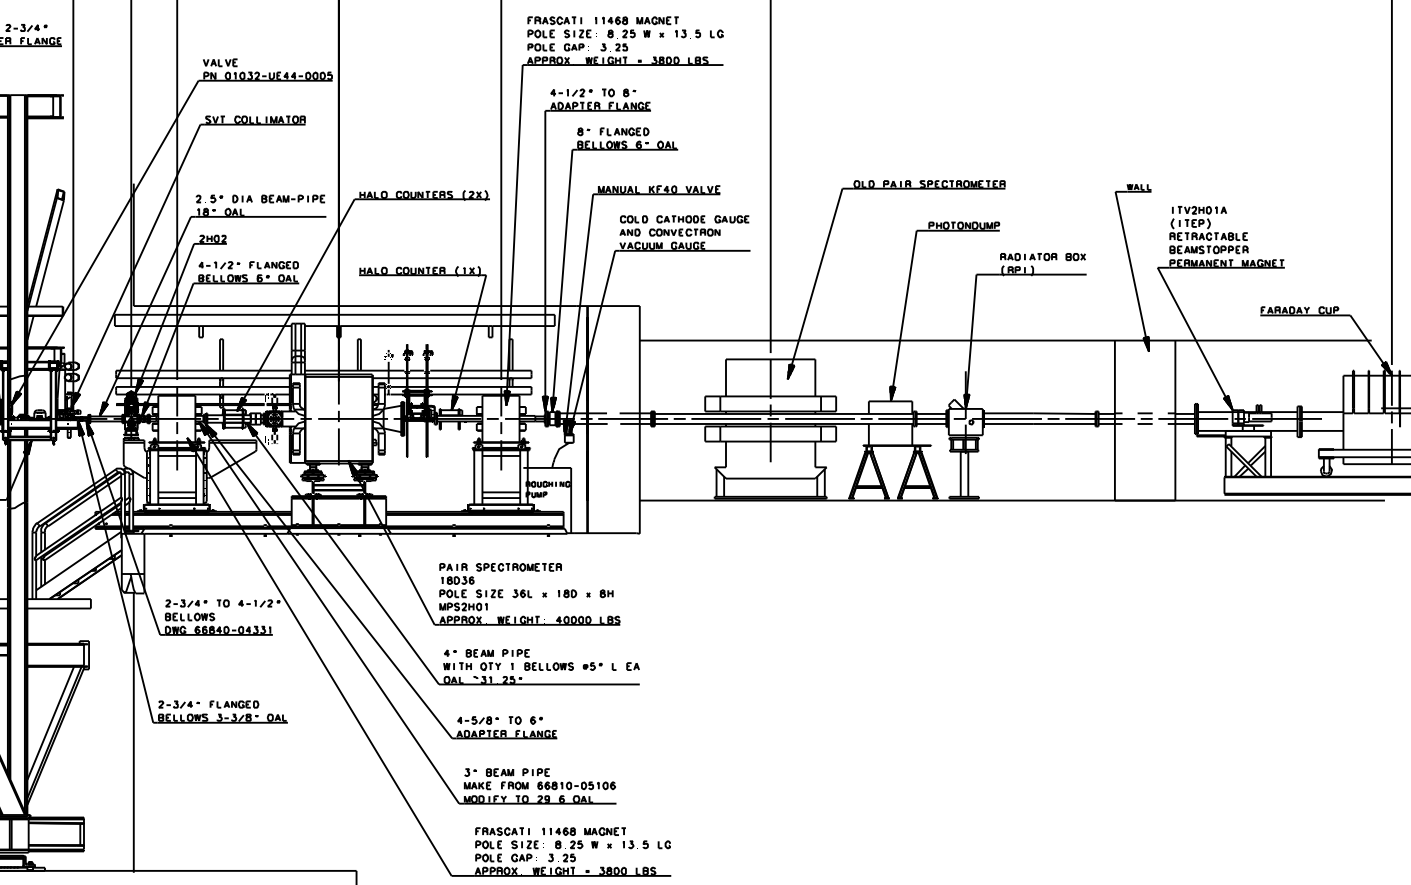
\includegraphics[width=\textwidth]{images/beamline.png}
    \caption{Configuration of the beam line during the HPS engineering run.}
    \label{fig:beamline}
\end{sidewaysfigure}

\section{Silicon Vertex Tracker}

\subsection{Layout}

The HPS SVT is comprised of two halves of six measurement layers encroaching the
beam plane as shown of Figure \ref{fig:svt_layout_render}. Each layer consist of a pair of
closely-spaced silicon planes with one of the planes oriented orthogonal to
the beam plane and the other at small angle stereo 
(see Table \ref{tab:svt_layout}).
\begin{figure}[h!t]
    \centering
    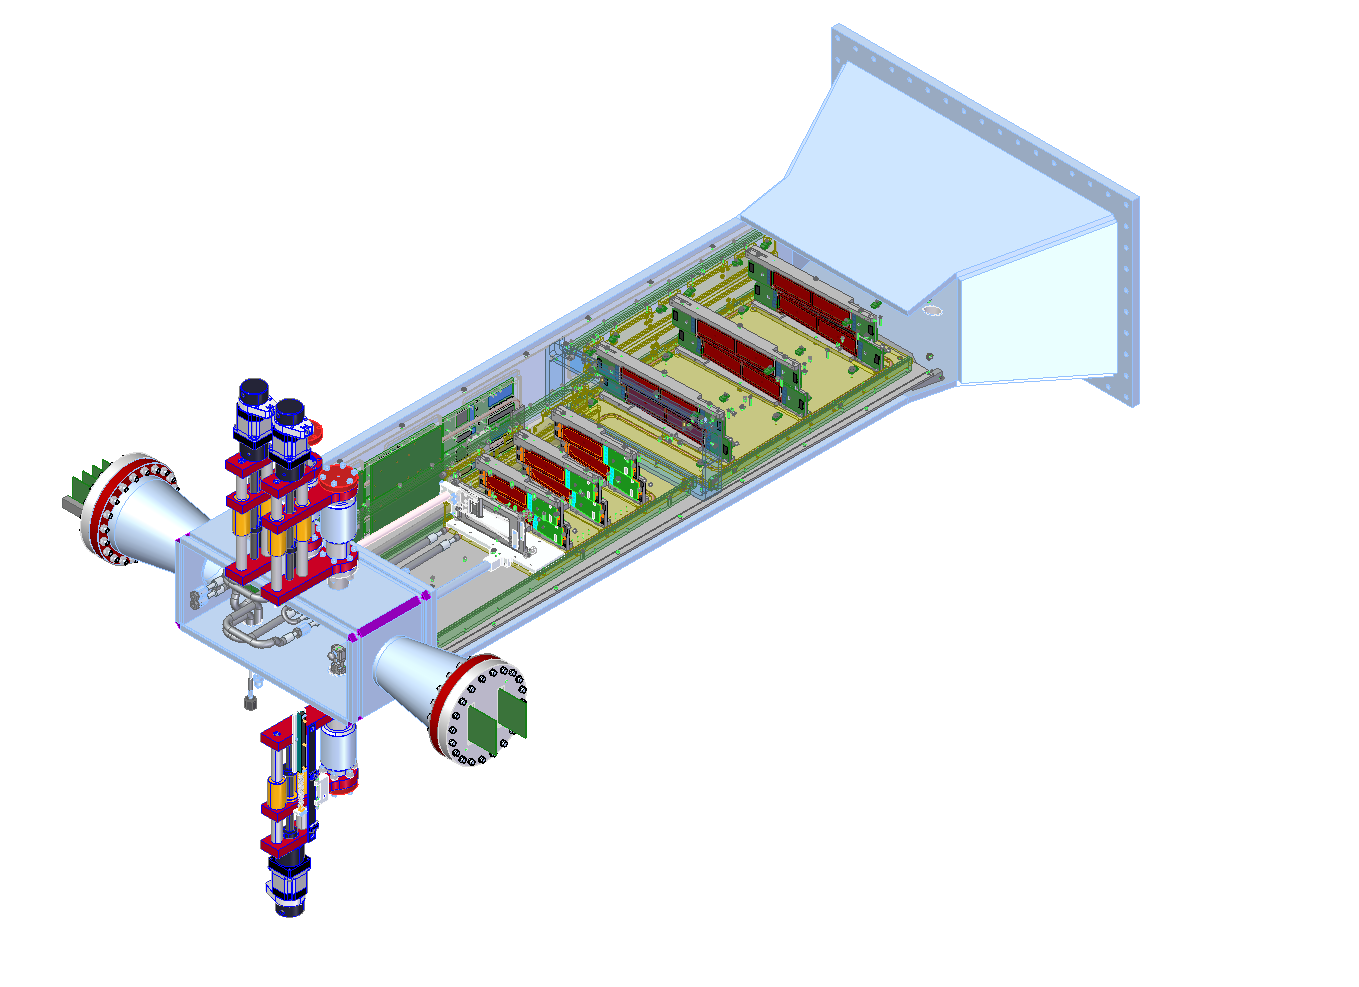
\includegraphics[width=0.9\textwidth]{images/svt_layout_render.png}
    \caption{A rendered view of the Silicon Vertex Tracker inside of the pair
             spectrometer vacuum chamber.}
    \label{fig:svt_layout_render}
\end{figure}
This allows
for the measurement of both the vertical and horizontal coordinate of a hit, in turn, 
enabling full 3D hit reconstruction.  

The first three layers consist of a single sensor of coverage above and below
the beam plane and use a stereo angle of 100 mrad. In order to better match the
% needs a sentence explaining why 100 mrad stereo was used.  According to the
% proposal, it balances acceptance against vertexing resolution.
acceptance of the Ecal, the coverage of the last three layers is two sensors 
wide and use a stereo angle of 50 mrad.  The choice of a 50 mrad angle for the
last three layers instead of 100 mrad was meant to break the degeneracy that
results in fake tracks
due to ghost hits in layers with the same stereo angle.  It must be noted that
only five layers are needed to match the full acceptance of the Ecal, however,
an improvement in the momentum resolution was observed with the addition of 
another layer.  In total, the SVT makes use of 36 sensors, which amounts to 
23,004 channels.

Since heavy photons are produced very forward, and the opening angle of their 
decay products goes as $\sim m_{A}/E_{0}$, sensitivity to low mass heavy photons
requires
the tracker layers to be as close to the beam plane as possible.  When deciding
the distance of the first layer to the beam, several effects needed to be taken
into consideration. These include the extent of the beam halo, the amount of 
radiation damage that is expected to be incurred from the Coulomb scattering
of the primary beam as well as radiative secondaries, the ability to resolve 
hits with pileup present and being capable of doing pattern recognition in a high 
occupancy environment.  With all of this in mind, it was determined that the 
closest tolerable distance was 15 mrad, putting the active edge of layer 1 
at 0.5 mm from the beam center. In simulation, this corresponds to 1\% occupancy
of strips closest to the beam plane of layer 1.

% I should talk about the positions as surveyed.
%The SVT layout is summarized in Table \ref{tab:svt_layout}. \textbf{Talk about
%the survey}.

%%%%%%%%%%%%%%%%%%%%%%%%%%%
%%% Table of SVT layout %%%
%%%%%%%%%%%%%%%%%%%%%%%%%%%
% I should use the survey positions here.
%\begin{table}[t]
\begin{sidewaystable}
    \centering
    \begin{tabular}{lcccccc}  
        \toprule
        \textbf{Layer} & \textbf{1} & \textbf{2} & \textbf{3} & \textbf{4} & \textbf{5} & \textbf{6} \\
        \midrule
        \midrule
        $z$ position from target (cm)    & 10 & 20 & 30 & 50 & 70 & 90 \\
        Stereo angle (mrad) & 100 & 100 & 100 & 50 & 50 & 50 \\
        Bend plane resolution ($\mu$m) & $\approx$6 & $\approx$6 & $\approx$6 & $\approx$6 & $\approx$6 & $\approx$6 \\
        Non-bend plane resolution ($\mu$m) & $\approx60$ & $\approx60$ & $\approx60$ & $\approx120$ & $\approx120$ & $\approx120$ \\
        Nominal dead zone in $y$ (mm) & $\pm$ 1.5 & $\pm$ 3.0 & $\pm$ 4.5 & $\pm$ 7.5 & $\pm$ 10.5 & $\pm$ 13.5 \\ 
        Material budget & .7\% & .7\% & .7\% & .7\% & .7\% & .7\% \\
        \bottomrule
    \end{tabular}
    \caption{The layout of the HPS SVT.}
    \label{tab:svt_layout}
\end{sidewaystable}
%%%%%%%%%%%%%%%%%%%%%%%%%%%

\subsection{Sensors}

At the energies at which HPS operates, the uncertainty in both the mass and
vertex resolutions are dominated by multiple Coulomb scattering in the first 
few layers.  This made it important to choose a sensor technology that would 
minimize the material budget of the SVT modules, especially since the material
budget of the sensors dominates the total material budget of the SVT modules.
Furthermore, the need to place the SVT in close proximity
to the beam plane made it necessary to choose sensors which are highly tolerant
to radiation.  With these 
considerations in mind, a readily available batch of silicon microstrip sensors,
initially manufactured for the D0 Run IIb upgrade, were found to satisfy all 
necessary requirements \cite{D0Collab:2003}.

The sensors were manufactured by Hamamatsu Photonics Corporation on 
$\langle 100 \rangle$ crystal rotation silicon and are $p^{+}$ on $n$-bulk, 
single sided, AC-coupled and polysilicon-biased. The cut dimensions of the 
sensors are $100 \times 40.34$ mm$^{2}$ with an active area of 
$98.33 \times 38.34$ mm$^{2}$. They are $320 \pm 20 \mu$m thick and have a sense
(readout) pitch of 30 (60) $\mu$m. The sensor specifications are summarized on 
Table \ref{tab:sensor_specs}.
\begin{table}[t]
    \centering
    \begin{tabular}{lr}
        \toprule
        Cut dimensions (L$\times$W)     & 100 mm x 40.34 mm \\
        Active area (L$\times$W)        & 98.33 mm x 38.34 mm \\
        Readout (Sense) pitch           & 60 (30) $\mu$m \\
        \# Readout (Sense) strips       & 639 (1277) \\
        Breakdown voltage               & $>1000$ V \\
        Depletion voltage               & $> 130$ V \\
        Bias Resistor Value             & $0.8 \pm 0.3$ M$\Omega$ \\
        AC Coupling Capacitance         & $>12$ pF/cm \\
        Total Interstrip Capacitance    & $< 1.2$ pF/cm \\
        Defective Channels              & $<1$ \% \\
        \bottomrule
    \end{tabular}
    \caption{Specifications of the sensors used for the HPS SVT.}
    \label{tab:sensor_specs}
\end{table}

Over the lifetime of the HPS detector, the sensor strips closest to the beam 
plane are expected to see $>10^{15}$ electrons per cm$^2$.  The radiation
damage the sensors are expected to incur due to the large electron flux,
will lead to an increase in both the leakage current and the voltage required to 
fully deplete the sensor.  It was then beneficial to choose a sensor technology
that can be operated at high bias voltage in order for them to remain fully
depleted even after irradiation. In fact, previous studies have shown that 
sensors that may be operated to 1000 V can tolerate a dose of 
$1.5 \times 10^{14}$ 1 MeV neq/cm$^2$ \cite{Fretwurst:2002vb}.  Since the damage
incurred by electrons with energies less than 10 GeV is a factor $\sim$ 30 less
than 1 MeV neutrons \cite{Rashevskaya:2002nd},
then ensuring all sensors can be biased to 1000 V will ensure that the sensors
will be able to withstand the expected flux of electrons over the lifetime of
HPS. 


Before being considered for use for the SVT modules, all sensors were electrically 
characterized.  Specfically, the leakage current was measured as a function
of bias voltage up to a maximum bias of 1000 V.  During these test, leakage 
currents of less than 500 nA were observed.  The measured IV curves for a subset
of sensors can be seen on Fig. \ref{fig:sensor_iv_curves}.  Only sensors whose
leakage current did not uncontrollably increase (i.e. breakdown) before reaching
a bias of 1000 V  were considered for use in HPS.
\begin{figure}[h!t]
    \centering
    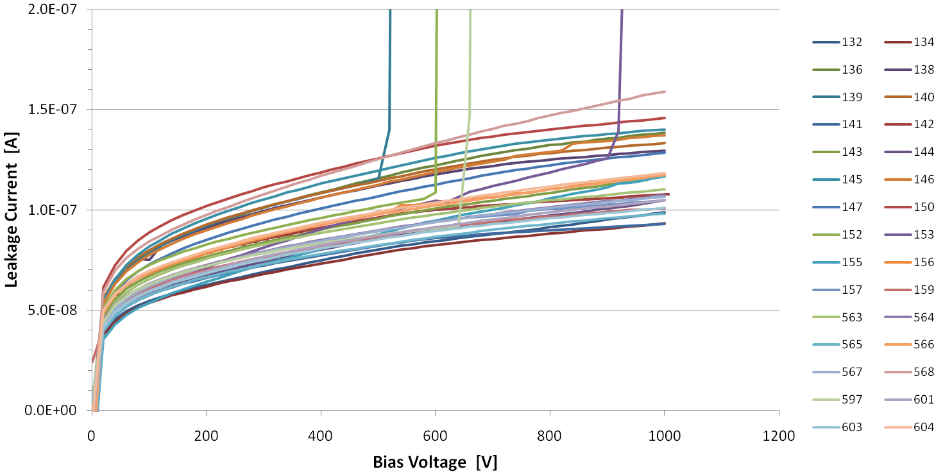
\includegraphics[width=\textwidth]{images/sensor_iv_curves.png}
    \caption{Measured IV curves for a subset of sensors used by HPS.}
    \label{fig:sensor_iv_curves}
\end{figure}

\subsection{Readout} \label{subsec:readout}

The sensors are continuously read out using the APV25 readout chip developed for
the Compact Muon Solenoid detector at the Large Hadron Collider 
\cite{Raymond:2000ey}. The APV25 has 128 channels, with each channel consisting
of a charge sensitive pre-amplifier coupled to CR-RC shaping amplifier and 192
cell deep analog pipeline.  A schematic of a single channel is shown on 
Fig. \ref{fig:apv25_schem}.
\begin{figure}
    \centering
    \includegraphics[width=0.9\textwidth]{images/apv25_channel_schematic.png}
    \caption{A schematic of a single channel of the APV25 readout chip.}
    \label{fig:apv25_schem}
\end{figure}

When a particle traverses a sensor, it generates a charge signal which is 
processed by APV25 amplifier chain.  As shown on Figure \ref{}, the shaper output
is continoulsy sampled at 40 MHz into the analog pipeline. If a trigger is 
received, the cells of interest along the pipeline are marked for read out. 
Since the trigger decision cannot happen instantenously in time, the position
along the pipeline from which the reading out of samples will begin is 
programmable.  Given that only 160 pipeline cells out of the 192 are used
to buffer samples, the readout delay or latency can be as long as 4 $\mu s$.
The remaining 32 cells along the pipeline are used to buffer samples that are
waiting to be read out.

The samples  are readout out by the Analog Pulse Shape Processor (APSP) which
can operate in two modes: peak mode and deconvolution mode.  In peak
mode, only a single pipeline cell is read out corresponding to the maximum 
value of the CR-RC shape.  In deconvolution mode, three consecutive samples are
read out allowing for the reconstruction of the shaper output.  The output of 
the APSP is then sent to a 128:1 multiplixer which then makes the raw data 
frames.  An example of the output data frame is shown on Figure \ref{}.

During the engineering run, the APV25's used the nominal  operating points with
a shaping time of 50 ns.  The nominal operating points are summarized on Table
\ref{tab:apv_spec}. The high occupancies expected during the engineering
run meant that overlapping of hits or ``pile-up'' were a concern.  In order to 
mitigate this problem, the APV25's were operated in deconvolution allowing 
the reconstruction of the shaper output.  Furthermore, 
with each Ecal trigger, the APV25's were sent two consecutive trigger signals 
allowing readout of six consecutive samples instead of three.  The trigger
latency was then adjusted such that two samples before the signal were readout, 
allowing the shape of the pileup pulse to be captured.  This was used to remove
any effects of pileup from the signal pulse.  This is illustrated on Figure 
\ref{fig:apv_shape}.
\begin{figure}
    \centering
    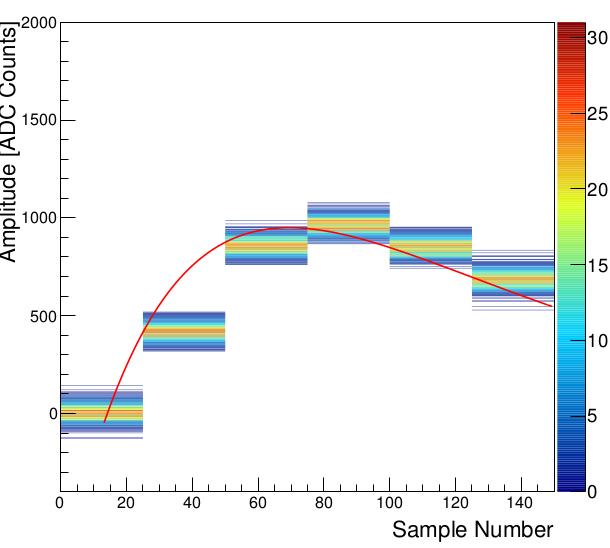
\includegraphics[width=0.9\textwidth]{images/sideB_response_ch535.png}
    \caption{The signal shape observed during the engineering run.}
    \label{fig:apv_shape}
\end{figure}
\begin{table}[t]
    \centering
    \begin{tabular}{l|c}
        \hline
        \hline
    \end{tabular}
    \caption{APV25 specs used during the engineering run.}
    \label{tab:apv_specs}
\end{table}

\subsection{Modules}

Each sensor requires 5 APV25 chips in order to readout all channels.  The 5 
APV25 chips are mounted on a FR4 electronic readout board, or hybrid, containing
filtering for the high voltage bias and a temperature sensor.  Since the pitch
of the APV25 and the sensors are similar, the chips were wirebonded directly to
the sensors without the need of a pitch adapter.

For layers 1-3 a ``half-module'' consist of a single sensor and hybrid glued 
onto a polyimide-laminated carbon fiber composite backing.  The half-modules 
for layers 4-6 consist of two sensors glued end onto the carbon fiber backing 
with hybrids on either side of them.  Due to space constraints, the hybrids used
by layers 4-6 have smaller footprint.  In order to further minimize the 
amount of material, a window is machined in the carbon fiber leaving the middle
of the sensor exposed. Fig. \ref{fig:l13_hm} and \ref{fig:l46_hm} show both a layer 1-3 and 4-6 
half-modules.
\begin{figure}
    \centering
    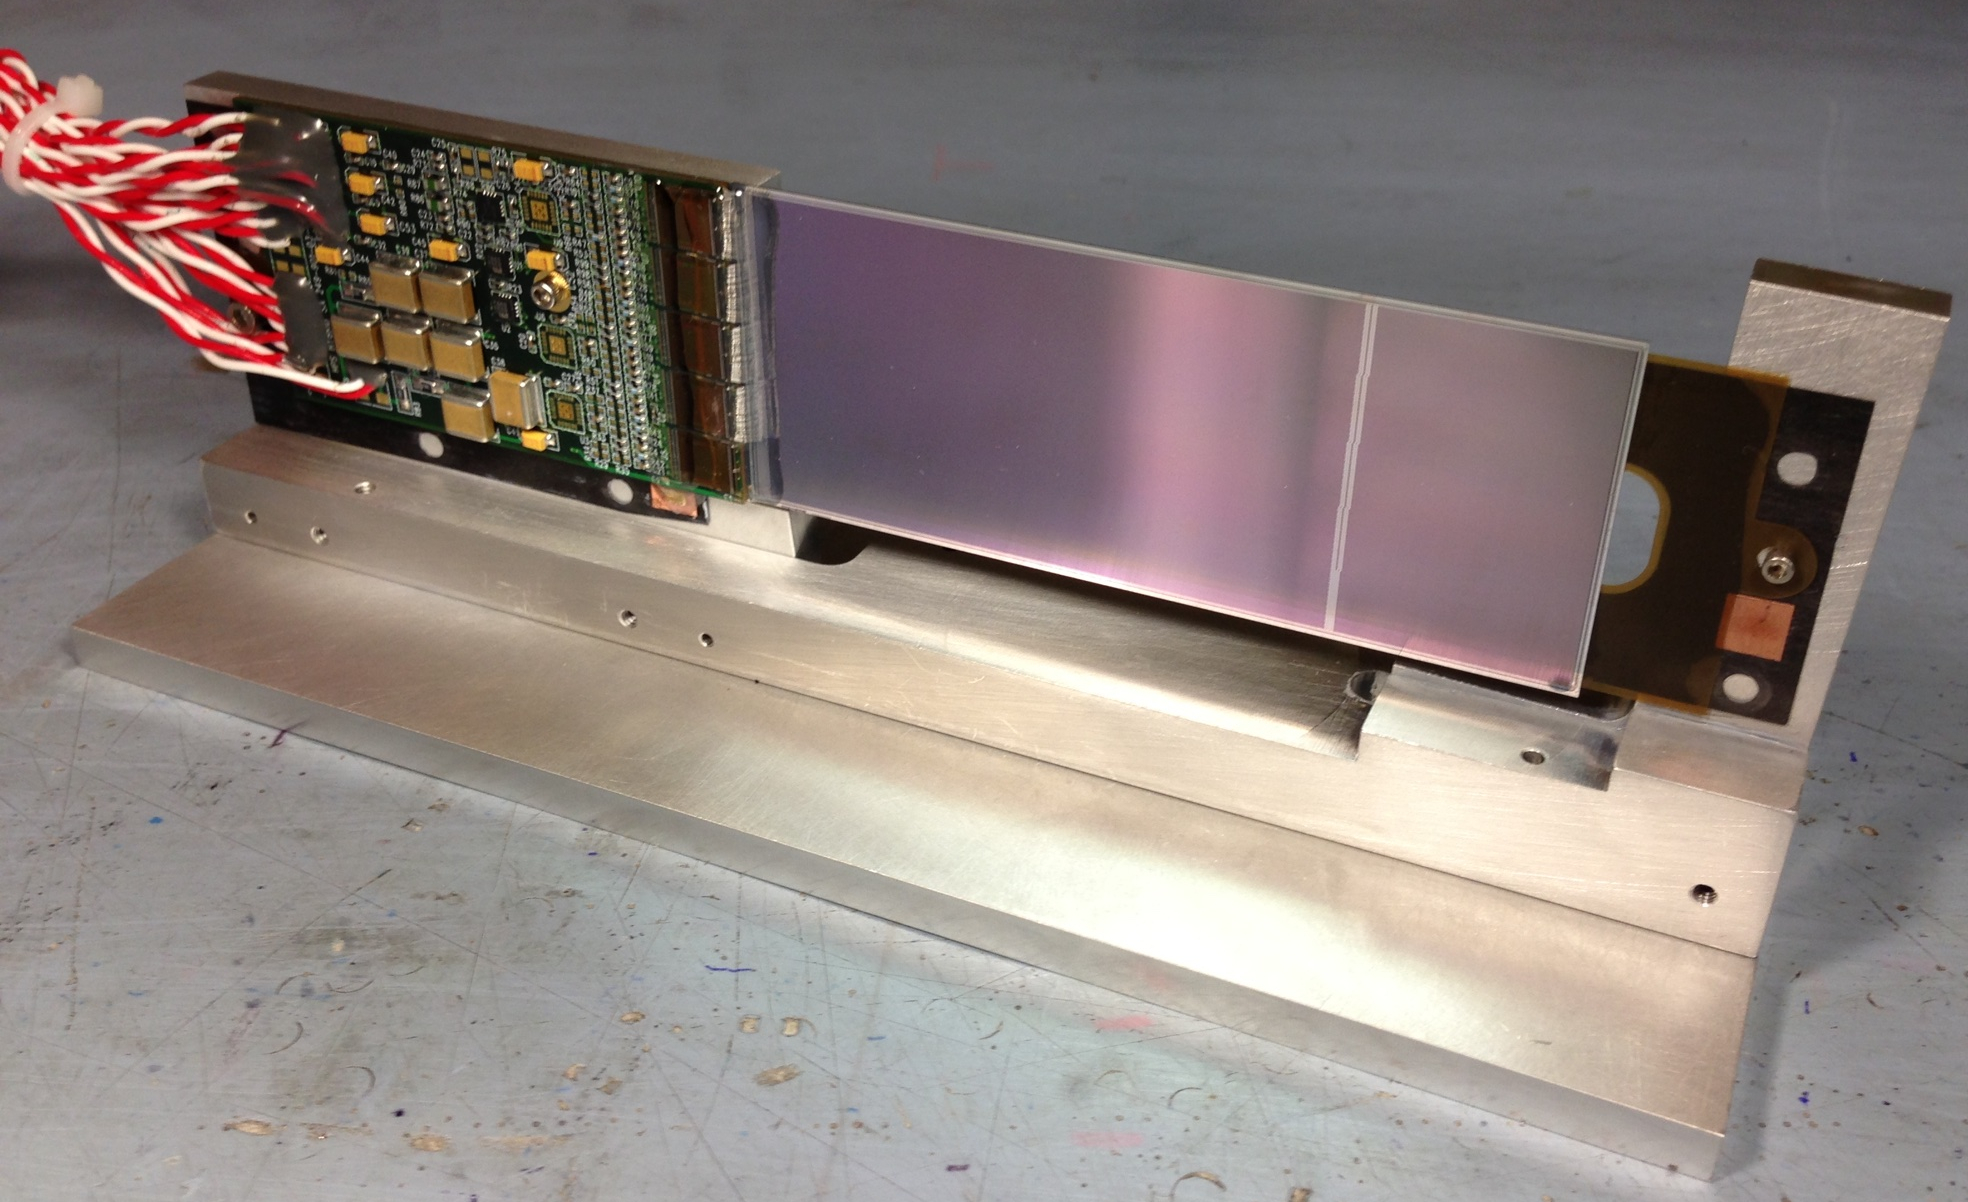
\includegraphics[width=0.9\textwidth]{images/l13_half_module.jpg}
    \caption{A layer 1-3 half-module used by the SVT. }
    \label{fig:l13_hm}
\end{figure}
\begin{figure}
    \centering
    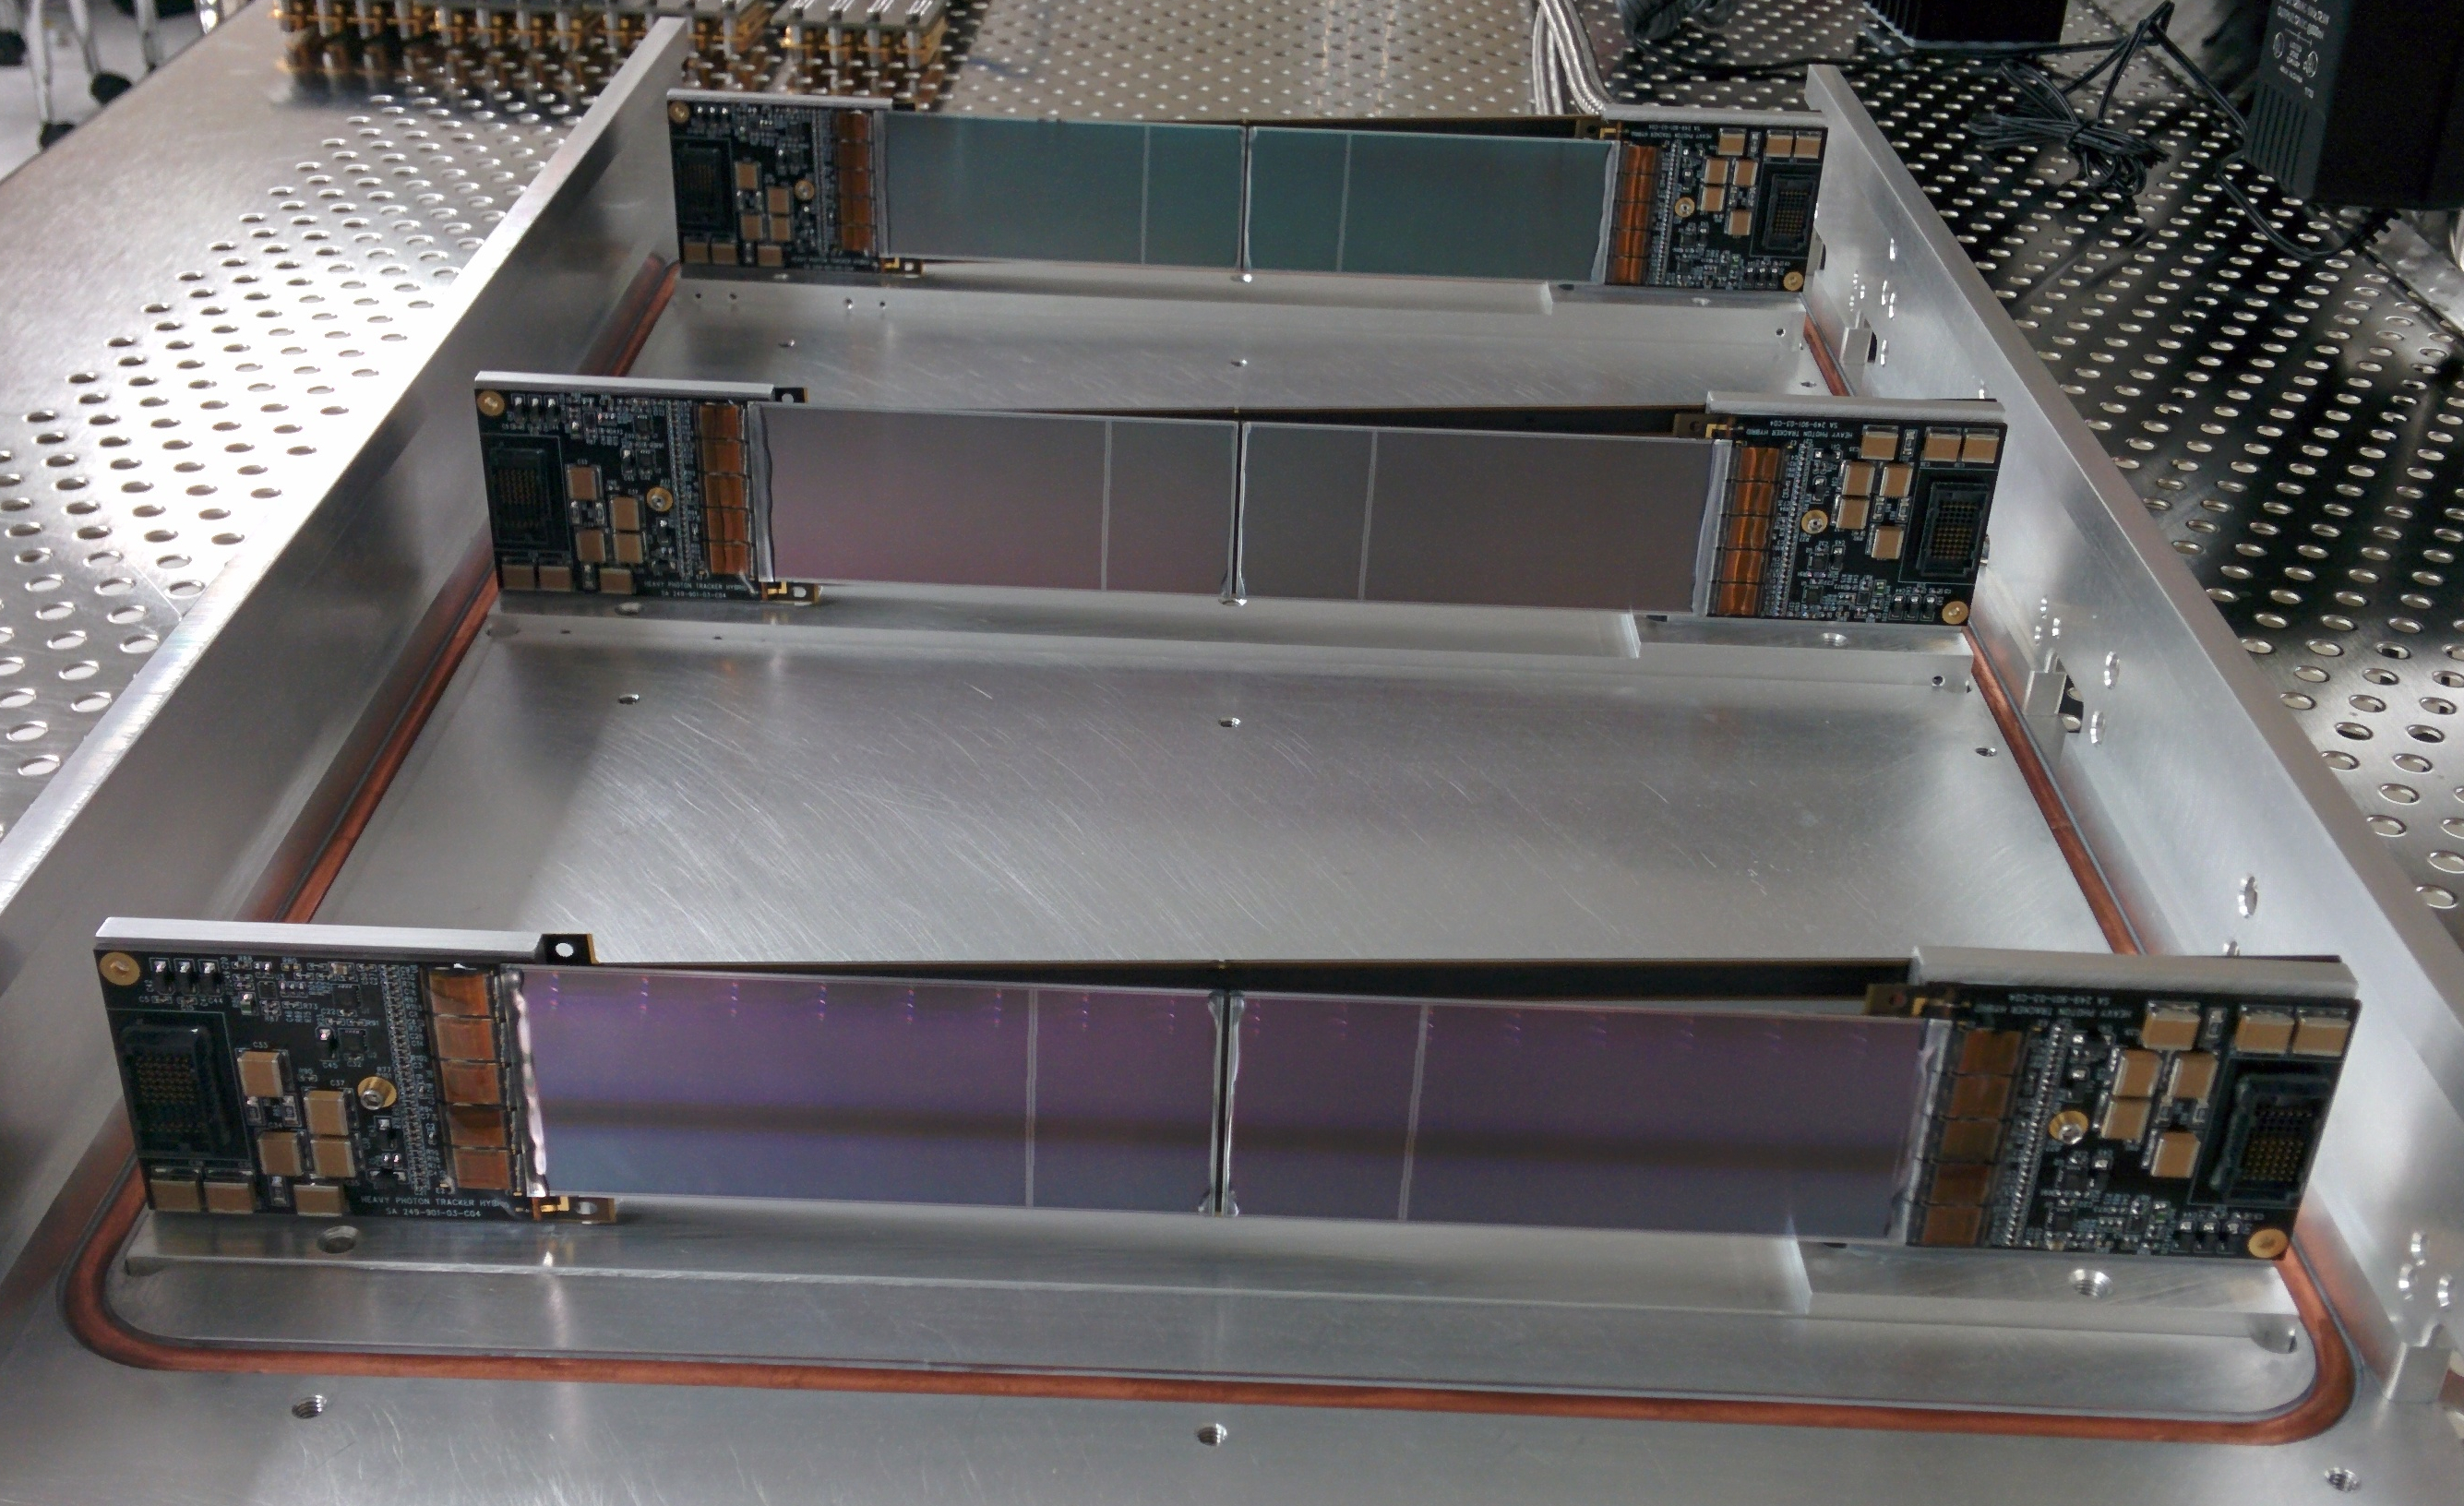
\includegraphics[width=0.9\textwidth]{images/l46_half_module.jpg}
    \caption{A layer 4-6 half-module used by the SVT. }
    \label{fig:l46_hm}
\end{figure}


\subsection{Mechanical Support, Cooling and Services}

...


\section{Electromagnetic Calorimeter}

The HPS Ecal is used as the primary trigger for the experiment as well as to
identify electrons and positrons.  It consist of two halves of lead-tungstate 
PbW0$_4$ crystals with each half mounted on an aluminum frame $\sim 137$ cm 
from the upstream edge of the analyzing magnet.  Each half is composed of five
layers of crystals with the four most outer layers consisting of 46 crystals and 
\begin{figure}
    \centering
    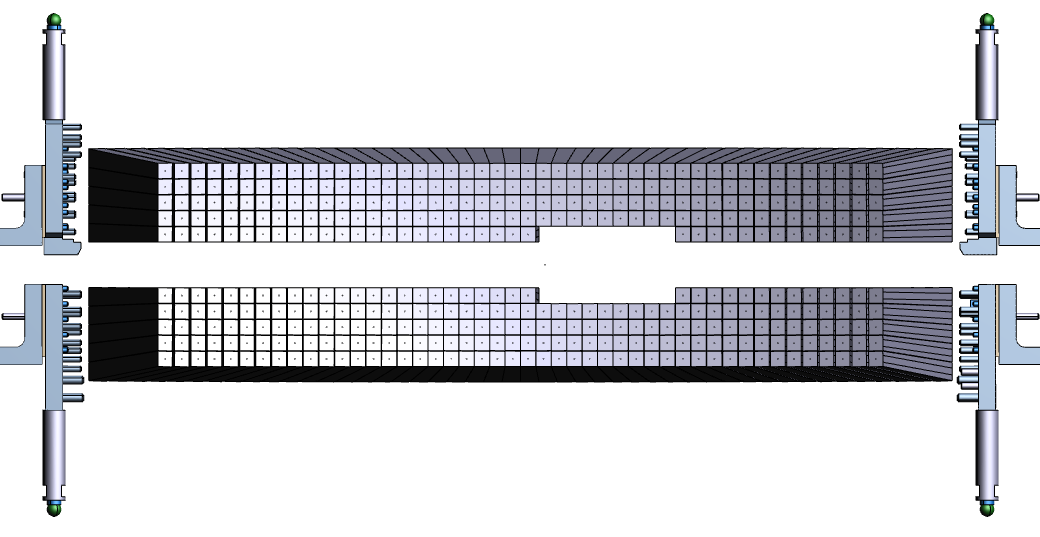
\includegraphics[width=0.8\textwidth]{images/ecal_layout.png}
    \caption{A rendering showing the arrangement of the Ecal crystals.  The Ecal
             is split into upper and lower modules in order to accommodate the 
             ``dead zone''.  The crystals removed from the first layer allow
             a larger opening for the outgoing electron and photon beams.}
    \label{fig:ecal_layout}
\end{figure}
the layer closest to the beam plane consisting of 37. The removal of the 9 
crystals from the inner layer was necessary to allow the outgoing electron and
photon beams to pass through unimpeded.  Each half is enclosed in a temperature
controlled environment held at 1$^{\circ}$ F which encroaches on the Ecal 
vacuum chamber.

Each of the crystals is 16 cm long and trapezoidal in shape with a front face
dimension of $1.3 \times 1.3$ cm$^2$ and a back face dimension of $1.6 \times
1.6$ cm$^2$.  In order to maximize the light yield, the crystals were wrapped
in VM2000 non-metallic reflector film. A Hamamatsu S8664-1010 Avalanche 
Photodiode (APD) with a photosensitive area of $10 \times 10$ mm$^2$ was glued
to the back of each crystal and used to read out the signals collected by the
crystals.  
\begin{figure}
    \centering
    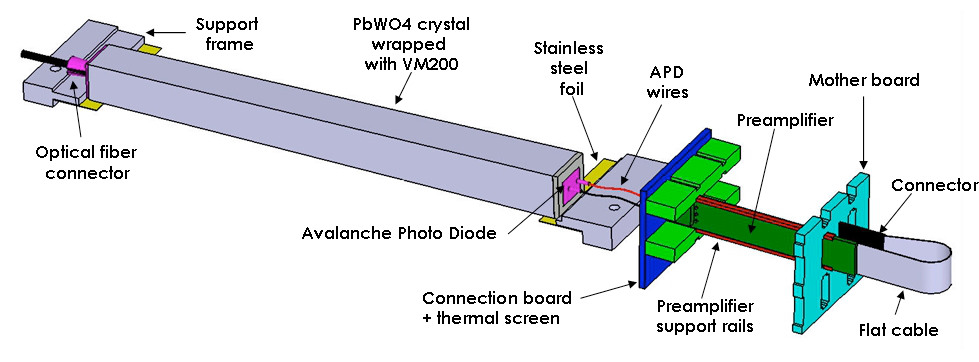
\includegraphics[width=0.8\textwidth]{images/ecal_crystal.png}
    \caption{Rendered view of an HPS Ecal module consisting of a 16 cm PbW$_4$
             crystal, Avalanche Photodiode and preamplifier board.}
    \label{fig:ecal_crystal}
\end{figure}

\section{Trigger and Data Acquisition}

\textbf{Write overview ...}

\subsection{Ecal DAQ}

\subsection{SVT DAQ}
% Need to discuss the hybrid design for both layers 1-3 and 4-6.
% 1) Need to mention why different wiring was used for the different parts of 
% the SVT.
%
%

After a trigger is received, the differential current signals 
from each of the APV25's are transferred to a total of 10 Front End Boards (FEB)
to undergo digitization and further processing. (Add figure?) As discussed in 
section (), the signals from layers 1-3 are transferred to the FEB's via 
Teflon-coated twisted pair wires while those emerging from
layers 4-6 use twisted pair magnet wire.  The use of twisted pairs reduces
crosstalk between the lines as well as electromagnetic interference.

At the FEB's, the differential current signals are first converted to a voltage
by a pre-amplifier circuit to match the dynamic range 
of the AD9252 14-bit analog to digital converter (ADC). The ADC samples the 
signal at 41.667 MHz and digitizes it to a value between 0 and 16384.  The 
digitized signals are then transferred to Xilinx Artix-7 field programmable
gate arrays (FPGA).  The signals are sent upstream by multi-gigabit transceivers.

Those signals which pass the threshold requirement are transferred through 
mini SAS wires to a board on the vacuum  where they undergo optical conversion.
The optical signal is then transferred over ~10 m fibers to the ATCA crate.


%\subsection{Ecal DAQ}

 % Maybe show an example of how the signal looks emerging from the APV?


